%%%%%%%%%%%%%%%%%%%%%%%%%%%%%%%%%%%%%%START PREAMBLE THAT IS THE SAME FOR ALL EXAMPLES
\documentclass{article}

\usepackage{Sweave}
\usepackage{graphicx}
\usepackage{tabularx}
\usepackage{hyperref}
\usepackage{natbib}
\usepackage{pdflscape}
\usepackage{array}
\usepackage{gensymb}
\usepackage{amsmath}
\usepackage{xr}

%\usepackage[backend=bibtex]{biblatex}
%Strongly recommended
  %put your figures in one place
%\SweaveOpts{prefix.string=figures/, eps=FALSE} 
%you'll want these for pretty captioning
\usepackage[small]{caption}

\setkeys{Gin}{width=0.8\textwidth}  %make the figs 50 perc textwidth
\setlength{\captionmargin}{30pt}
\setlength{\abovecaptionskip}{10pt}
\setlength{\belowcaptionskip}{10pt}
% manual for caption  http://www.dd.chalmers.se/latex/Docs/PDF/caption.pdf

%Optional: I like to muck with my margins and spacing in ways that LaTeX frowns on
%Here's how to do that
 \topmargin -1.5cm        
 \oddsidemargin -0.04cm   
 \evensidemargin -0.04cm  % same as oddsidemargin but for left-hand pages
 \textwidth 16.59cm
 \textheight 21.94cm 
 %\pagestyle{empty}       % Uncomment if don't want page numbers
 \parskip 7.2pt           % sets spacing between paragraphs
 %\renewcommand{\baselinestretch}{1.5} 	% Uncomment for 1.5 spacing between lines
\parindent 0pt% sets leading space for paragraphs
\usepackage{setspace}
%\doublespacing

%Optional: I like fancy headers
%\usepackage{fancyhdr}
%\pagestyle{fancy}
%\fancyhead[LO]{How do climate change experiments actually change climate}
%\fancyhead[RO]{2016}
 
%%%%%%%%%%%%%%%%%%%%%%%%%%%%%%%%%%%%%%END PREAMBLE THAT IS THE SAME FOR ALL EXAMPLES

%Start of the document
\begin{document}

%\SweaveOpts{concordance=TRUE}

\bibliographystyle{../refs/bibstyles/amnat.bst}% i moved a style file into the ospree git repo. feel free to add whatever style you like and update, lizzie! I don't have besjournals
\title{Shifts in Southern Resident Killer Whale Phenology in the Salish Sea}
\date{\today}
\maketitle
\author{A.K. Ettinger, C. Harvey, J. Samhouri, B. Hanson, C. Emmons, J. Olson, E. Ward}
\maketitle  %put the fancy title on
%%%%%%%%%%%%%%%%%%%%%%%%%%%%%%%%%%%%%%%%%%%%%%%%%%%
\par 
\emph{Target journal(s)}: Global change biology, Journal of Applied Ecology %, Marine Ecology Progress Series, not currently written for a short-form journal but perhaps consider PNAS?
\section* {Introduction}
\par Phenology, or the timing of biological activities such as migration, growth, and reproduction, can have dramatic implications for fitness \citep{lane2012,chuine2010}. Consumer phenology that is out of step with its resource phenology can cause increased mortality %\citep{lamaris2018} 
or reduced reproductive success \citep{post2007}. The critical nature of these ``matches'' or  ``mismatches'' was originally described for fish and zooplankton \citep{hjort1914,cushing1974,cushing1975}, and has received renewed scientific interest as phenological shifts have been increasingly observed in conjunction with recent climate change \citep{durant2007}. 

\par Despite its importance, phenology of many organisms, even those of conservation concern, remains poorly understood and is rarely quantified, especially for marine organisms. A recent meta-analysis found that shifts in marine phenology are at least as dramatic as those observed in terrestrial systems (e.g., - 4.4 $\pm$0.7 days per decade) \citep{poloczanska2013}. The abundance of critical resources is more often a focus of natural resource management, yet the timing of resource peaks can be at least as important to consumers \citep{hipfner2008}.
 %JS: I am also thinking that some of the ecological literature on resource pulses could be helpful here, eg Yang et al 2008, 2010
\par Southern resident killer whales (SRKWs, \emph{Orcinus orca}) are a federally endangered population that spends time in the inland waters of Washington State, USA, and British Columbia, Canada.  They have received widespread scientific and public attention in recent years as their numbers have declined\citep[e.g., Seattle Times articles,][]{lusseau2009,larson2018, olson2018}. Insufficient prey availability is believed to be one of the primary threats to this population, along with vessel traffic and pollutants \citep{krahn2007,lusseau2009,hanson2010}. SRKWs differ from many orca whales in that their primary prey are salmon (\emph{Oncorhynchus} species), especially Chinook salmon \citep[\emph{Oncorhynchus tshawytscha}][]{hanson2010}. SRKWs use inland waters to hunt for their prey when they are aggregated and locally highly abundant. Salmon have a distinct seasonality to their migration patterns,  and SRKWs also vary seasonally in their use of inland waters: they travel between summer and winter core areas that can be separated by thousands of kilometers \citep{balcomb1986,krahn2005}. 
\par In recent decades, the abundance and phenology of the favored prey of SRKWs, salmon, has shifted in the western United States \citep{weinheimer2017,reed2011,ford2006,satterthwaite2014}(add Nelson for chinook hatchery release timing), though patterns vary by species and location. We would therefore expect SRKW phenology to have shifted during this time, if prey is a primary driver of their activity in inland waters. If SRKW phenology has not shifted at a rate consistent with phenological shifts in their prey, this mismatch could exacerbate the low prey availability they experience. 
%\par Add a paragraph about monitoring of whales? Quantifying changes in the timing of SRKW activity in inland waters over the pst 40 years is challenging because monitoring effort has increased during this time \citep{olson2018, strebel2014}. 
\par Here, we seek to quantify seasonal variation in SRKW activity and the extent to which these seasonal patterns have shifted over the past four decades.  %CH: I think the overall blueprint is good here; this lays out the objectives and context pretty clearly and will benefit from the additional forthcoming details and perhaps some effort to sharpen the stick a bit and make a clearer case of the urgency faced by the SRKW pop and therefore the importance of this work
Specifically, we ask:
\begin{enumerate}
\item Has the timing of SRKW activity (phenology) shifted in the Salish Sea? 
\item If there have been phenological shifts in SRKW activity, do these shifts coincide with shifts in phenology of their prey, salmon (\emph{Oncorhynchus} species)?
\end{enumerate}

\section* {Methods}
\subsection*{Focal species description}
Southern resident killer whales are a population of killer whales that inhabit coastal waters from central California to northern British Columbia.  During the summer months they are often seen in inland water's of Washington and southern British Columbia (Fig. \ref{fig:phenplot}). Sourthern residents are considered distinct from another population of fish-eating killer whales, known as the northern resident killer whales (NRKWs), whose distribution is further north, and from co-occuring `transient' killer whales, which feed primarily on marine mammals (Bigg 1982). Southern resident killer whales have declined dramatically since the 1970s, and are now listed as endangered under the Canadian Species at Risk Act (SARA) and the US Endangered Species Act (ESA). Threats to this population include small population size, chemical contamination, disturbance from boat traffic, and insufficient prey availability (Holt et al. 2009, Lusseau et al. 2009, Noren et al. 2009, Williams et al. 2009, Ward et al. 2009, Ford et al. 2009). The SRKW population is composed of three subgroups, or pods, identified as J, K, and L, which are matrilineally related, coheisve and stable social groups. Individuals rarely disperse from their natal pods (Bigg et al. 1990).
\subsection* {Data}
\par \underline{Southern resident killer whales}: To quantify SRKW seasonal phenology over time, we used the OrcaMaster Database for Whale Sighting Data (Whale Museum), comprised of data from five main sources, including public sightings networks (e.g., OrcaNetwork), commercial whale watch data, and scientific surveys (e.g., SPOT data from satellite tracking units) \citep{olson2018}. We used data from 1978-2017, because prior to this time there was no dedicated effort to track SRKW presence in the region \citep{olson2018}. We used these sighting data to quantify %first observation day-of-year (DOY, the first date on which one or more pods of SRKWs were observed in a given region) and last observation DOY (the lasst date on which one or more pods of SRKWs were observed) 
detection of SRKWs in the two core areas: the Central Salish Sea, used primarily by SRKWs from May through September, and Puget Sound proper, visited by SRKWs most commonly from September through January \citep{olson2018}. We used these seasonal definitions because they are most aligned with mean SRKW seasonal activity patterns over time (Fig \ref{fig:phenplot}).  We also quantified number of whale days (i.e. days on which whales were observed) within a season and year for each region. 

\par \underline{Salmon}: To quantify potential shifts in SRKW prey phenology over time, we used two datasets. We used adult salmon return ('escapement') data for coho, chum, and chinook salmon in Washington state (https://wdfw.wa.gov/fishing/management/hatcheries/escapement). Daily or weekly WDFW data are available for 67 streams going back to 1997 and include wild and hatchery counts. We selected sites located close to Puget Sound or the central Salish Sea (i.e.., within XX km) with the greatest available data (i.e., long time series with frequent monitoring), and with relatively large run sizes (range of average counts from trap estimates = 1,400-30,000 for chum, 621 - 11,500 for coho, and 550-13,350 for chinook.) We stress that the particular runs we chose may not be widely represented in SRKW diet, but they represent the best available data for salmon phenology in Washington state of which we are aware. 

\par We also used data from the Albion Chinook and Chum test fisheries, located  on the lower Fraser River at Albion, British Columbia, Canada (https://www.pac.dfo-mpo.gc.ca/fm-gp/fraser/docs/commercial/albionchinook-quinnat-eng.html), 80-90\% of the chinook salmon consumed by SRKWs appear to be from the Fraser River \citep{hanson2010}.

\subsection* {Analysis}
\underline{Southern resident killer whales}:
\par To identify trends over time in phenology for SRKWs in the Central Salish Sea and in Puget Sound proper, we summarized the number of whale days (days on which whales were observed), as well as first-, last-, and mean- observation dates from 1978 through 2017 in each region. 

\par We quantified pod-specific phenology for J, K, and L pods in the Central Salish Sea versus Puget Sound Proper using occupancy models. Occupancy models can estimate jointly species presence and detection probability (\emph{p},the probability of detecting at least one individual present at a site) by distinguishing true presence or absence, \emph{z} (a latent, unobservable state), from observed presence. Occupancy models are composed of a state submodel, which is the model for the ecological process of true presence or absence, and  an observation submodel, which links the observations (i.e., whether or not whales were seen) to the state model.
\par We fit a hierarchical model in which occupancy probability (psi) was a function of day of year (i.e., we did not fit a dynamic model, but a multi-year model,Royle and Kery 2007), with year and marine area as levels. Occupancy probability was modeled as a semi-parametric, smooth function of day of year (`\emph{day}')using flexible thin-plate spline regression modelling \citep{strebel2014}. We assumed \emph{z}, to be a Bernoulli random variable for which 0 signifies absence and 1 is presence. We modeled detection probability (\emph{p}) as a year- (`\emph{yr}') and marine area- (`\emph{area}') specific probability between 0 and 1. Thus, our occupancy model can be described by the following equations:

\par Observation model:
\begin{equation} 
y_{area,yr,day} \sim Binomial (T_{yr,day,area}, z_{yr,day} * p_{area,yr})\\
\end{equation}

\par State model:
\begin{equation} 
z_{yr,day} \sim Bernoulli (\mathrm{\Psi}_{yr,day})\\
\end{equation}

\par Occupancy models were fit in JAGS with R2jags \citep{su2015} in R, version 3.5.1 \citep{r2018}. We fit separate occupancy models within each region (and season, since seasonal use varies by region) for each pod, and extracted estimates of annual arrival, departure, and peak occupancy dates with each model. We defined arrival date as the earliest DOY within the season when occupancy probability exceeded 0.5; departure date was the latest DOY within the season when detection probability exceeded 0.5. (Using a threshold probability lower than 0.5 did not qualitatively alter observed trends, Figure SX.)

\par With increasing public awareness of the plight of SRKWs and with the rise of social media, there has been a dramatic increase in reported sightings of SRKWs since 1978 \citep{olson2018}. As a presence-only database, trends in the OrcaMaster dataset should be interpreted with care, since they could be due to shifts in effort as well as (or instead of) trends in SRKW activity. For this reason, we report all trends across two different durations: the full dataset (from 1978-2017) and recent years (2002-2017). We use 2002 as a cut-off, the avoid the included a sharp increase in sightings that occurred in 2001, likely influenced by the onset of internet-based sightings platforms that began that year \citep{olson2018}. Further, because the above occupancy models cannot fully statistically account for changes in effort over time, due to the presence-only nature of the data, we compared phenology estimates from the occupancy models to phenology observed at Lime Kiln state park from 1990 to 2017. This dataset represents a subset of the OrcaMaster database that was collected with consistent observer effort from May through September \citep{olson2018}.  

\underline{Quantifying effects of changes in effort}: (could move this to supp?)
\par To better understand how increased effort across the timeseries (i.e., increased numbers of sightings over time) may affect estimates of trends in phenology, we simulated data sets of whale presence during two seasons equivalent to those in our data set (summer, which was 1 May through 31 Sept, or 153 days, and fall, which was 1 October through 1 Feb, or 123 days). We used whale presence probabilities of 0.85 for the Central Salish Sea and 0.6 for Puget Sound (the means in our data set for each region) and kept it constant over 40 simulated years. We then created an observation data set, in which effort (the number of observations), varied. During the low effort time period (years 1-20), the number of observations had a mean of 15 per year for Puget Sound and 104 per year in the Central Salish Sea (matching the means for these regions from 1978-1997 in the OrcaMaster database).  During the high effort time period (years 21-40 in our simulated data set), the number of annual observations had a mean of 39 for Puget Sound and 133 for the Central Salish Sea (matching those in the OrcaMAster database from 1998-2017). We then calculated first- and last- observations dates for each simulated year. We ran these simulation 100 times and calculated the difference between the low effort and high effort time periods. We compared these to the mean differences first- and last-observation dates across time periods in the OrcaMaster database, for each region, to understand whether observed changes may be due to changes in effort over time, rather than changes in orca activity.\\
\underline{Salmon}:
\par We used hierarchical linear models to identify trends over time in first, median, peak, and last dates of salmon adult migration timing in Puget Sound proper. We treated distinct rivers and species, as well as hatchery versus wild types of the same species, as separate groups in our model. Our model allowed for different trends (slopes) across these separate troups, estimating both species-level responses (generally yielding more accurate estimates for well-represented groups), and the distribution from which they are drawn, yielding an estimate of the overall response across groups.

\section*{Results}
\par We found that SRKW phenology has shifted. Since 2002, estimated peak occurrence probability in the Central Salish Sea has gotten later for all three pods, at rates ranging from 0.88  to 2.71 days per year (Fig. 2). Trends across the full dataset (1978-2016) were also toward later peak occurrence probability, though they were less dramatic (Fig. \ref{fig:timeseries}) and the dramatic increase in effort has likely affected some of these trends (see Supplemental Materials for details).  In Puget Sound proper, there has not been a consistent linear trend in peak occurrence since 2002 for any pod (i.e., credible intervals around the slopes encompass 0). The trends across the full time dataset has been toward later peak occurrence for all three pods (Fig. 2). 
\par Coincident with these phenological trends, the number of whale days has also changed across the time-series (Fig. 3). Across the full dataset, the number of whale days has increased in both regions (and for all pods). At least some of these increasing trends are due to increased effort (see Supplemental Materials). Since 2002, the number of whale days has decreased in the Central Salish Sea, across all pods. 
\par We found that salmon phenology has shifted as well, though the patterns differ across regions (Fig. 4). In the central Salish Sea, the return timing of chinook in the Fraser River has delayed by 0.80 per year (80\% credible intervals: 0.5-1.1 days per year) for first-observations dates from 1980-2018 (Fig 4A).  Delays in peak return and median return dates are stronger (1.2 and 1.3 days per decade, respectively). In Puget Sound proper, where data were available across more streams and the preferred prey of SRKWs are more poorly understood, we observed a shift toward earlier returns (Fig. 4B).
\par
\section*{Discussion}
\par The timing of SRKW activity has shifted over the past 40 years, with recent trends differing from long-term trends. Changes in marine phenology have been widely reparted and are often attributed to climate change. Given the observational nature of the dataset, and that many factors have changed over the length of the dataset, it is impossible to definitely identify drivers of these shifts. There are many possible explanations for their shifting phenology, a few of which we discuss below.

\par Phenological shifts observed in SRKWs may be attributable to changes in their prey. Summarize changes in salmon abundance and phenology on the west coast. Our results are consistent with this...The timing of adult salmon returns has also shifted. Populations in the central Salish Sea are arriving later, whereas many populations in Puget Sound proper, especially hatchery-origin fish, are arriving earlier. Compare rates of change
%\par The timing of SRKW activity in central Salish Sea and in Puget Sound proper appears to be shifting in a manner that differs from shifts in salmon timing. This difference may lead to a mismatch between predator and prey that causes additional stress on SRKW populations, since the timing of resource availability can be as important as the amount of the resource \citep[Brianna's work,][]{hipfner2008}
\par Social reasons for shifts
\par Other global change factors: increased vessel traffic and other disturbances. increased fishing?
\par Absence data are valuable! Observer effort has shifted over time. Its great that so many people are outside looking for whales! Recommend collecting absence data too. This would allow for more robust analyses of whale distributions. Challenge is increased time/money required for database maintenance with this extra data.

\section*{Conclusion}

\section*{Questions}

\begin{enumerate}
\item Currently I report trends for both recent years (since 2002) and the full time series (1978-present). Would it be better to only report on recent years? (Justified using the rationale already described in the methods- internet based reports.)
\item Fig. 2: Do you prefer the data version (with whale days) or the modeled version (with probability of occurence, Fig. 2Alt)? If Fig. 2Alt, which timespans to include (2008-2017 vs 1998-2007 OR 2008-2017 vs 1978-2007)?
\item Fig. 3: Add linear trend to time series of peak occurence day of year or no?
\item Fig. 4: salmon: Do we want to show the coefficents from linear models (as shown) or curves of CPUE (similar to figure 2) or something else?
\item Fig. 5: Lime Kiln vs broader Central Salish Sea phenological patterns, as related to chinook in the Fraser River. Other ideas for how to handle this?
\item Color scheme- do you like the color scheme currently (blue vs pink) or would other colors be prettier or more intuitive or better for some other reason?
\item Include simulation methods and results only in supplement?
\item What else should we include in the supplement (see below for a start)?
\item Full year models or seasonal models?

\end{enumerate}
\section*{To Do}
\begin{enumerate}
\item Write Discussion (for 9/24/2019)
\item Supplemental Materials:
\begin{enumerate}
\item Time series of peak prob. occurence for K and L pods
\item Time series for first- and last- dates when occurrence probabilty is greater than 0.5 for J,K,L pods
\item Expected phenological change due to change in effort alone (simulations)- do this for the recent time span as well?

\end{enumerate}
\end{enumerate}
\bibliography{../refs/noaalib.bib}


\section* {Figures}

\begin{figure}[p]
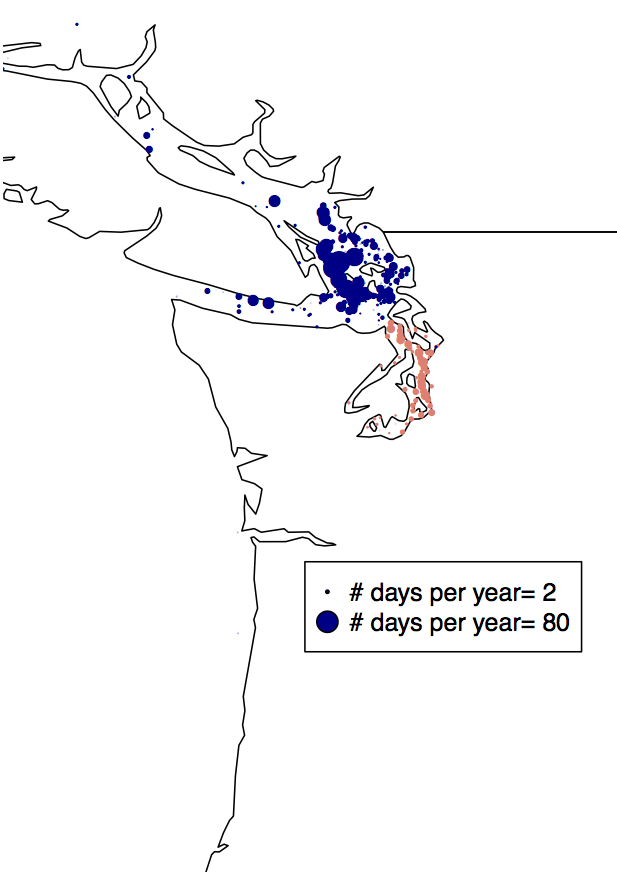
\includegraphics[width=0.5\textwidth]{../analyses/figures/OrcaPhenPlots/srkw_justmap_assumeSRKW_April1.png} 
\caption{\textbf{Southern resident killer whale activity varies across two broad regions: the Central Salish Sea and Puget Sound proper}. }
 \label{fig:map}
 \end{figure}
 
\begin{figure}[p]
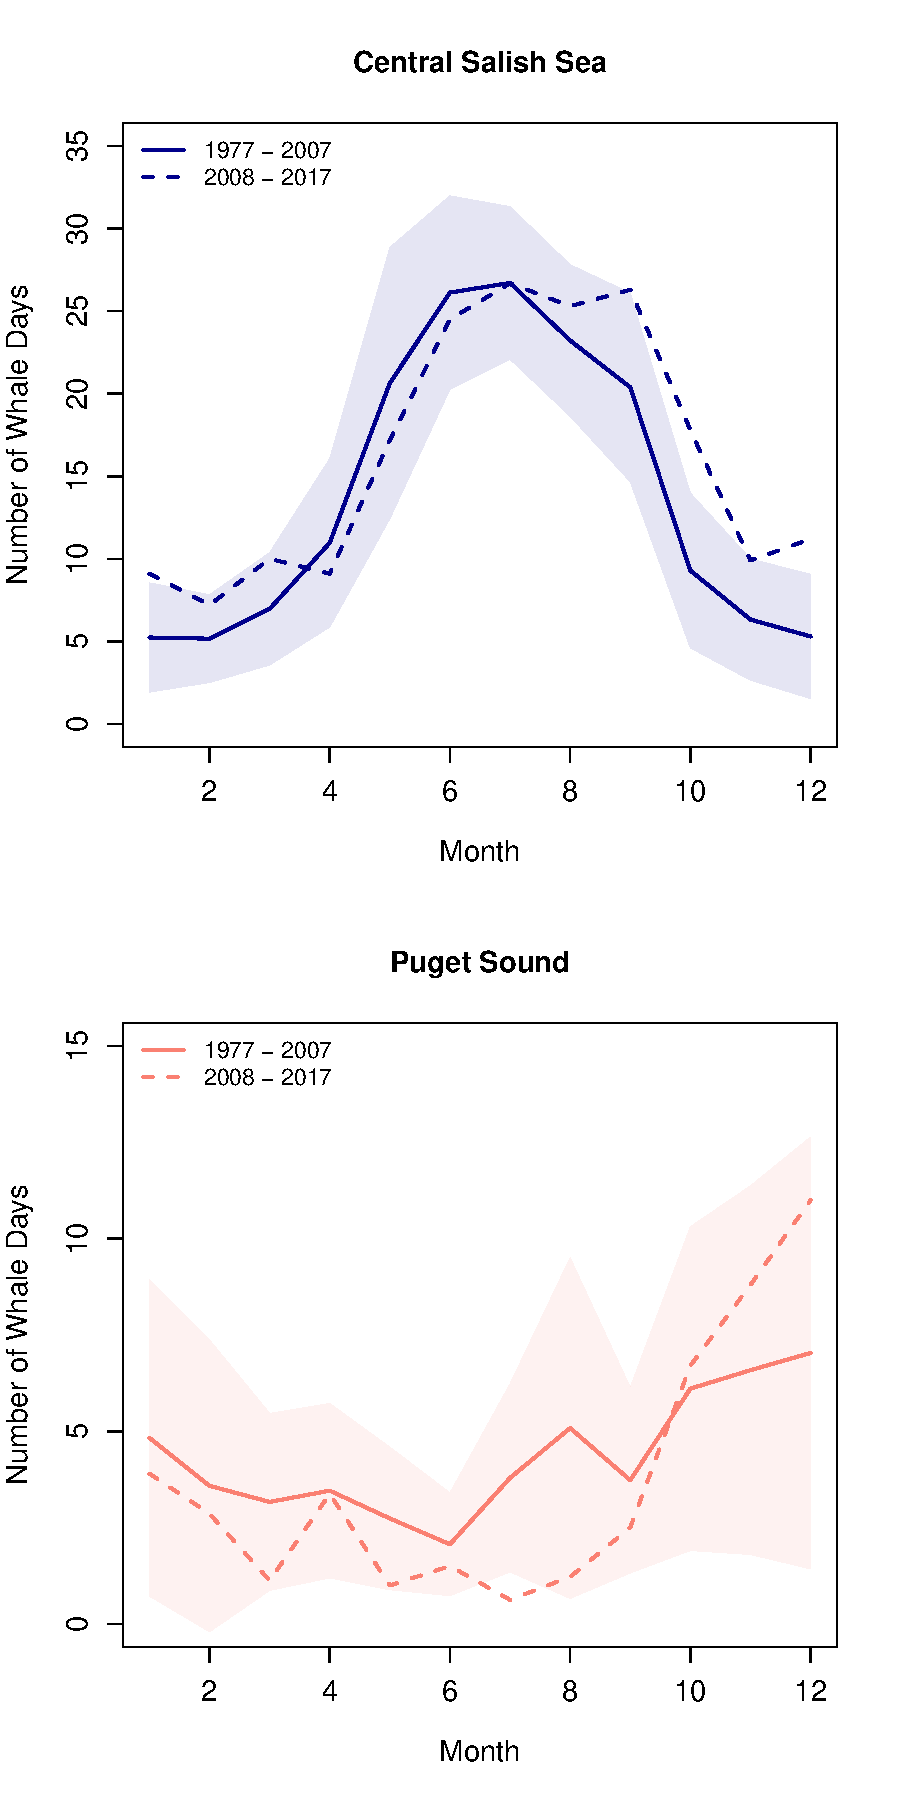
\includegraphics[width=0.6\textwidth]{../analyses/figures/OrcaPhenPlots/wdays_bymonth_earlylate_1976_assumeSRKW2regs.pdf} 
\caption{\textbf{Southern resident killer whale activity varies seasonally in the Central Salish Sea and Puget Sound proper} and this phenology has shifted later in recent years, particularly in the Central Salish Sea. Insets show linear trends in first-, peak-, and last- observation dates for J, K, and L pods, estimated from occupancy models. Error bars represent standard deviation.}
\label{fig:phenplot}
 \end{figure}


\begin{figure}[p]
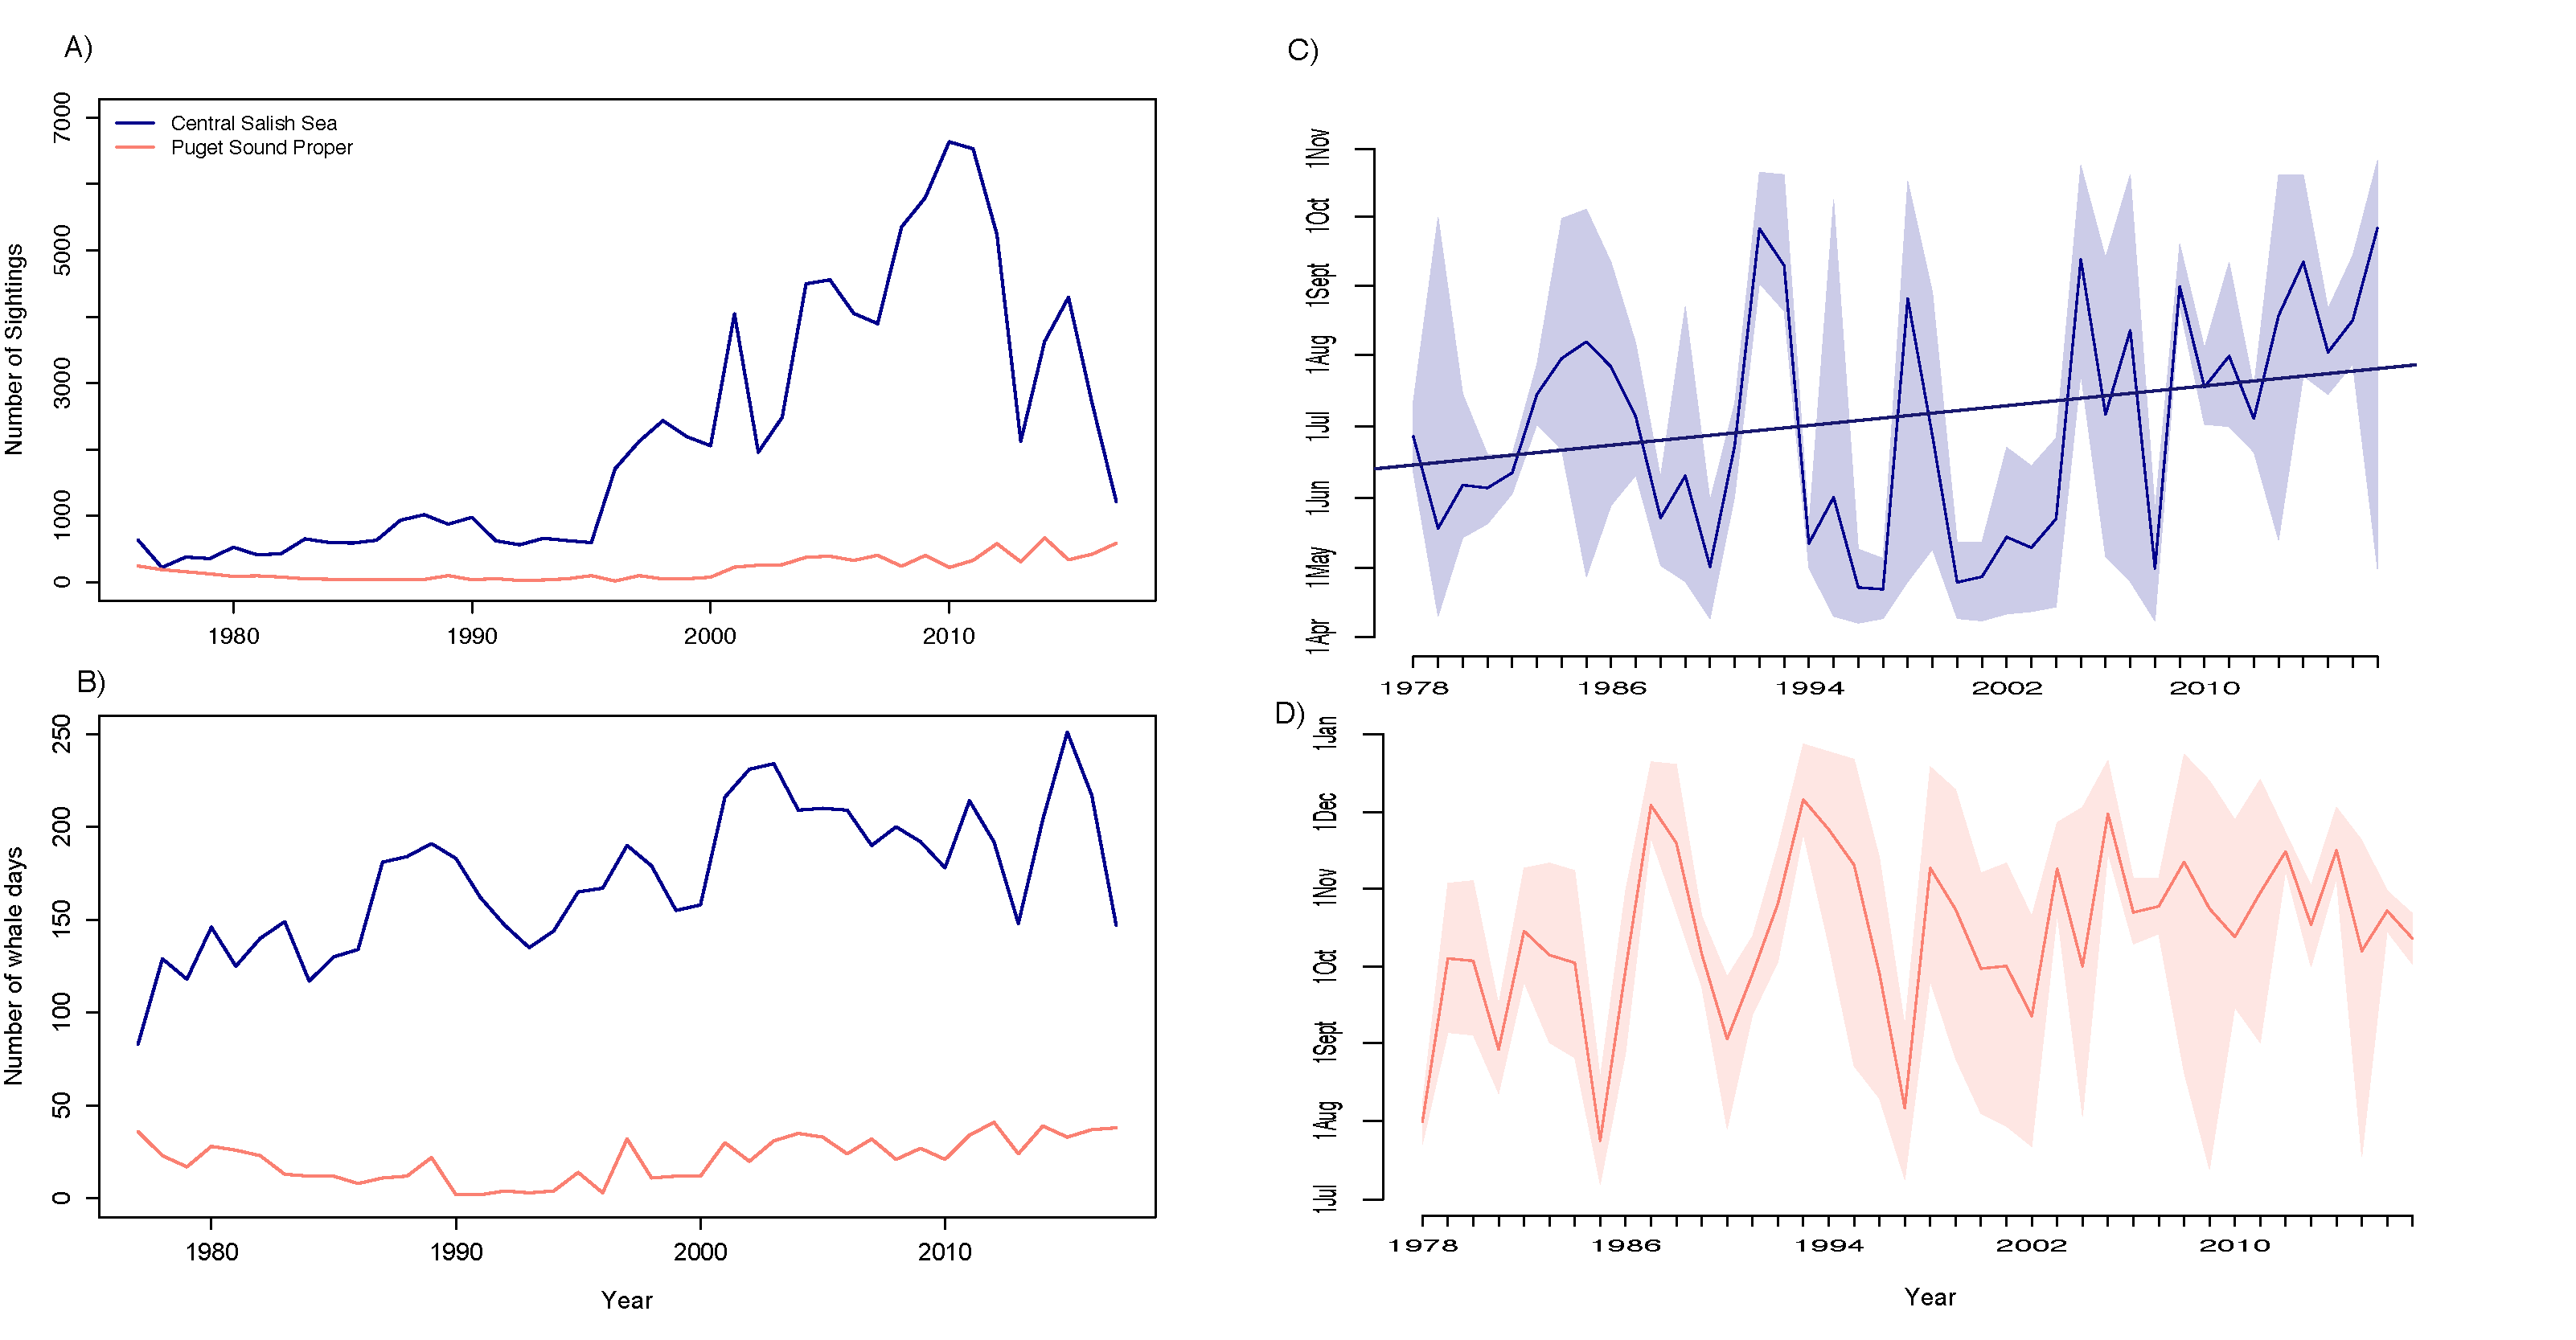
\includegraphics{../analyses/figures/OrcaPhenPlots/timeseries_1976_assumeSRKW2regs.pdf} 
\caption{\textbf{Long-term trends differ from recent trends} for whale sightings (A), whale days (B), and peak occurence probability in the Central Salish Sea (C) and Puget Sound proper(D). Occurrence probability for J pod is shown here; see Supplemental Materials for time series for K and L pods, as well as time series for other phenological estimates (i.e., first- and last- dates when occurrence probabilty is greater than 0.5). Shading represents 80\% credible intervals.}
 \label{fig:timeseries}
 \end{figure}
 

\begin{figure}[p]
\includegraphics[width=0.8\textwidth]{../analyses/figures/salmon_shifts_lmm.pdf} 
\caption{\textbf{Trends in first-, peak-, mid-, and last- observation dates for salmon} in the Fraser River Albion test fishery (upper panel), and across 17 different species/rivers in Puget Sound proper}
 \label{fig:shifts}
 \end{figure}

\begin{figure}[p]
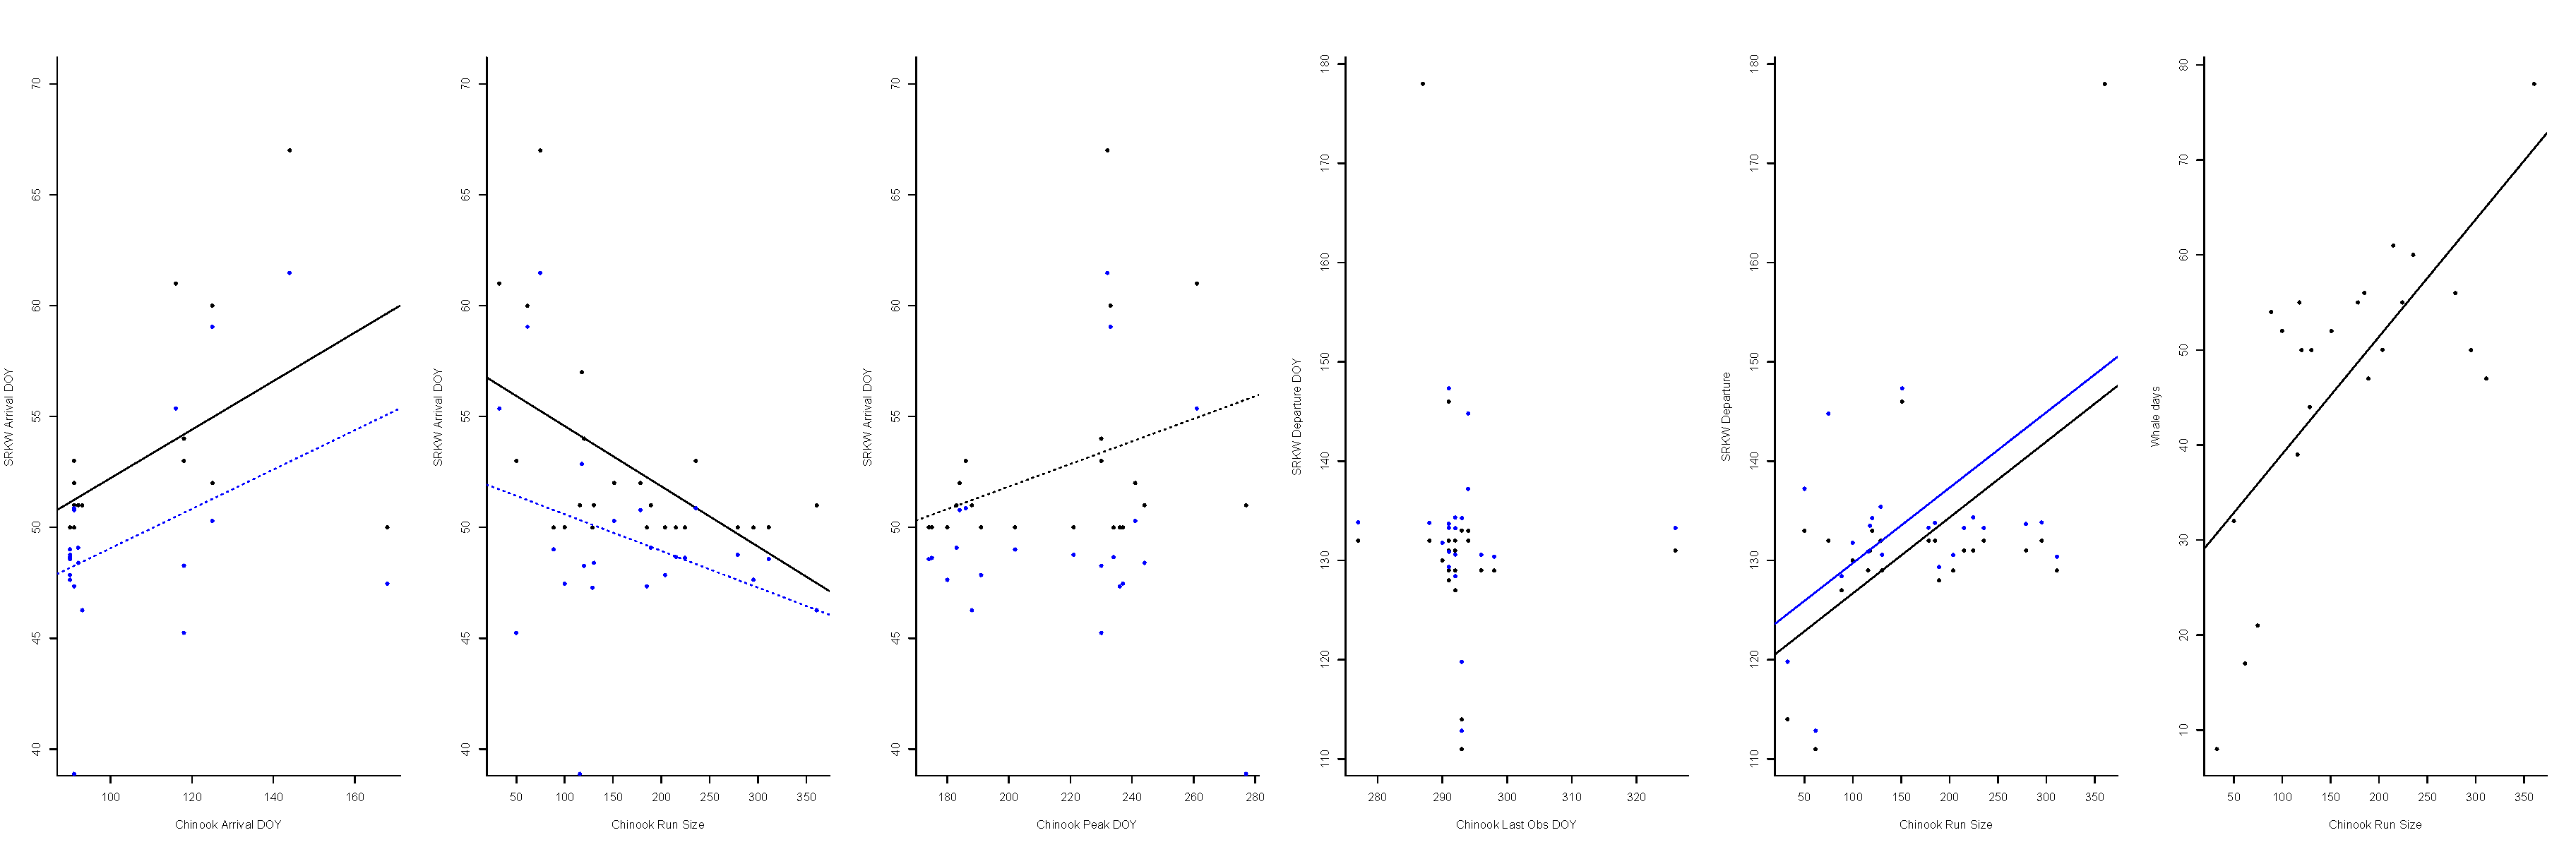
\includegraphics[width=0.8\textwidth]{../analyses/orcaphen/figures/lime_albchin.pdf} 
\caption{\textbf{SRKW phenology is related to estimated chinook phenology (A) and run size (B,C)}, for Lime Kiln State Park, a SRKW observation site in the central Salish Sea with a consistent data collection effort from 1994-2017 (from May through October,A). Chinook phenology and run size was estimated from the Fraser River Albion test fishery data. Phenology of the Central Salish Sea region as a whole appear to be less related to the patterns of this particular test fishery data, for many possible reasons (see Supplemental Materials for details).}
 \label{fig:shifts}
 \end{figure}

\end{document}
